\documentclass[10pt]{sigplanconf}

\usepackage{amsmath,amssymb, latexsym}
%\usepackage[noend]{algorithmic}
%\usepackage{algorithm}
\usepackage{program}
%\usepackage{pstricks}
\usepackage{graphicx}
\usepackage{wrapfig}
\usepackage{enumerate}
\usepackage{hyperref}
\def\url{}
\usepackage{subfigure}
\usepackage{epsfig}
\usepackage{epic}
\usepackage{eepic}


% command to end a proof or definition:
\def\qed{\rule{0.4em}{1.4ex}}

% space at the beginning of an environment:
\def\@envspa{\hspace{0.3em}}
\def\@sa{\hspace{-0.2em}}
\def\@sb{\hspace{0.5em}}
\def\@sc{\hspace{-0.1em}}
\def\sk{\smallskip}		% space before and after theorems

\newtheorem{notation}{Notation}{\itshape}{}
%\newtheorem{theoremstar}{Theorem}{\bfseries\upshape}{\itshape}
%\newtheorem{@protheo}{Theorem}

%\newenvironment{theorem}[1]{\begin{@protheo}{\rm \bf #1}\it}{\end{@protheo}}
%\newenvironment{proposition}[1]{\begin{@protheo}{\rm \bf #1}\it}{\end{@protheo}}

%\newtheorem{remark}{Remark}{\bfseries\upshape}{\rm}
%\newtheorem{definition}{Definition}{\bfseries\upshape}{\itshape}
% this is from the lazy_abstraction paper
%\newtheorem{notation}{Notation}{\itshape}{}
\newtheorem{theoremstar}{Theorem}{\bfseries\upshape}{\itshape}
\newtheorem{@protheo}{Theorem}
\newenvironment{theorem}[1]{\begin{@protheo}{\rm \bf #1}\it}{\end{@protheo}}
\newtheorem{remark}{Remark}{\bfseries\upshape}{\rm}
\newtheorem{definition}{Definition}{\bfseries\upshape}{\itshape}
\newtheorem{proposition}{Proposition}{\bfseries\upshape}{\itshape}
\newtheorem{lemma}{Lemma}{\bfseries\upshape}{\itshape}
\newtheorem{corollary}{Corollary}{\bfseries\upshape}{\itshape}
\newtheorem{invariant}{Invariant}



\newcounter{ex}
\stepcounter{ex}

\newenvironment{example}{\vspace{0.05in} \noindent {\sc Example \arabic{ex}: }}{\stepcounter{ex} \hfill $\Box$ \vspace{0.05in} }
%\theoremstyle{remark}
%\newtheorem{@proex}{Example}
%\newenvironment{example}[1]{\begin{@proex}{\rm \bf #1}}{\end{@proex                      }}
%\newtheorem{example}{Example}

\def\mynote#1{{\sf $\clubsuit$ #1$\clubsuit$}}

% comment environment
% comment.sty
% 25-Oct-89
% By Ed -- modified from verbatim in /usr/loca/lib/tex82/latex.tex

% \begin{comment}
% \end{comment}

\makeatletter

\begingroup \catcode `|=0 \catcode `[= 1
\catcode`]=2 \catcode `\{=12 \catcode `\}=12
\catcode`\\=12 |gdef|@xcomment#1\end{comment}[|end[comment]]
|endgroup

\def\@comment{\let\do\@makeother \dospecials\catcode`\^^M=10\def\par{}}

\def\begincomment{\@comment\@xcomment}

\makeatother

\newenvironment{comment}{\begincomment}{}


%%%%%%%%%%%%%%%% general macros

\def\set#1{{\{ #1 \}}}

%%%%%%%%%%%%%%%% paper specific macros
\def\Next{\hspace{4pt}\raise 3pt \hbox{\circle{7}} \hspace{4pt} }
\newcommand{\dia}{{\raisebox{-0.2ex}{$\Diamond$}}}
\newcommand{\PastDiamond}                                     % past diamond
     {\mbox{\rm\makebox[0em][l]{$\dia$}\makebox[0.8em]{--}\hspace{0.05em}}}

\def\create{{\mathsf{create}}}

\def\alloc{{\mathsf{alloc}}}
\def\access{{\mathsf{access}}}
\def\delete{{\mathsf{delete}}}

\def\acquire{{\mathtt{acq}}}
\def\release{{\mathtt{rel}}}

\def\alias{{\mathsf{alias}}}
\def\mayalias{{\mathsf{mayAlias}}}
\def\mustalias{{\mathsf{mustAlias}}}

\def\code#1{\texttt{#1}}

%%%%%%%%%%%%%%%%%%%%%%%%%%%%%%%%%%%%%%%%%%%%%
\sloppy

\begin{document}
\title{Static Checking for Dynamic Resource Management \\ in Sensor
  Network Systems}

\authorinfo{\mynote{PUT IN NAMES}}


\maketitle

% -*- tex-main-file: "main.tex" -*-

\begin{abstract}
%
\noindent 
Many sensor network systems expose general interfaces to system
developers for dynamically
creating and manipulating resources of various kinds.
%
While these interfaces allow programmers to accomplish
common system tasks simply and efficiently,
they also admit the potential for programmers to mismanage resources,
for example through
leaked resources or improper resource sharing. 
%
We describe a static analysis algorithm and tool that 
brings the safety of static resource management to
systems that dynamically manage resources.
Our analysis is based on the observation that programmers
often use implicit {\em ownership} schemes
to correctly manage dynamic resources.  In such a scheme, each
resource has a unique owner, who has both the capabilities to
manipulate the resource and the responsibilities to use the resource
properly and 
to dispose of it eventually.
Our tool checks resources at compile time for violations of
this ownership discipline.
%

We apply our tool to ensure proper management
of dynamically allocated memory in programs written on top of
SOS, a sensor network operating system.
%
We have evaluated the tool on all historical versions of all user
modules in the SOS CVS repository, as well as on the SOS kernel
itself.  
%
Our tool generated
%
88 warnings of which 16 were real errors when checking user modules and
28 warnings of which 2 were real errors when checking the kernel,
% 
demonstrating the tool's utility for practical sensor network systems.
%
\end{abstract}

\section{Introduction}
\label{sec:intro}

Networked embedded systems, or sensor networks, are finding ubiquitous
application in densely sampling phenomena --- from structural
properties of buildings to wildlife behavior --- that were previously
difficult or impossible to observe.  Like embedded systems, sensor
networks operate in resource and energy constrained environments with
minimal operating system support.  However, unlike traditional
``dedicated'' embedded applications, sensor network applications are
reprogrammable, and applications may change in the field.  For this
reason, sensor network applications can benefit from operating system
support for general-purpose system abstractions.

A useful class of system abstractions provides facilities to
dynamically manipulate system resources.  
%
% Another important class of abstractions are those that facilitate
% changing the owner of a resource.
%
Such abstractions can simplify application development and allow an
application to naturally and efficiently respond to the changing needs of its
environment.  
%
% Several platforms for sensor networks provide a form of dynamic
% resource management.  
%
For example, TinyOS~\cite{TinyOS} uses a buffer-swapping protocol 
between components for
efficient sharing of statically allocated buffers.  
The SOS operating system~\cite{sos} supports dynamic
allocation of memory, while MANTIS OS~\cite{abrach03mantis} supports
both dynamic memory allocation and thread creation.
Frameworks built on
top of sensor network systems also include components that make
resources dynamically available to other parts of the system.  
An example of this form of dynamic resource 
management is the
VanGo~\cite{greenstein05vango} framework's buffer pool for
TinyOS. 

%
% NOTE: With the addition of buffer swapping in TinyOS added above, is
% this paragraph still needed?
%
% While especially important for the proper management of dynamic
% resources, this kind of ownership model is also useful for managing
% static resources.  For example, TinyOS lacks support for dynamic
% memory allocation, but statically allocated buffers are often
% transferred among components for efficiency reasons.  TinyOS employs a
% split-phase approach to message passing~\cite{TinyOS}: a message
% pointer is passed via a call to {\tt Send.send}, and the sender
% receives the {\tt Send.sendDone} event when message transmission has
% completed.  The calling component should not modify the message
% pointer in any way until receiving the {\tt sendDone} event.
% Ownership is a natural protocol for guaranteeing this behavior:  the
% calling component transfers ownership of the pointer to the callee
% upon a {\tt send} call and regains ownership upon the {\tt sendDone}
% event~\cite{ownershipthread}.


While the ability to manipulate resources increases the expressiveness
of sensor network applications, this expressiveness can be a
double-edged sword.  Improper management of resources can lead to
subtle errors that can affect both the correctness and efficiency of
applications.

For example, consider the architecture of a simple sensor-network
sense and send application.
%, shown in Figure~\ref{fig:surge-dataflow}.
Like many sensor-network applications, this application can be
arranged for a dataflow architecture:  raw sensed data captured at the
sensors moves through various filters
% (via the {\tt surge} module)
before being forwarded to a base station.
% (via the {\tt tree routing} module).  
In order to naturally and efficiently implement the message passing,
data buffers are 
%  dynamically allocated as necessary and 
passed by
reference between system modules.
% rather than by copying.

If incorrectly implemented, this style of data sharing can lead to
serious errors.  First, a module may access a (dangling) reference to
data that has been passed on and possibly freed downstream. 
%
This is dangerous because
%
the low-end processor hardware used in current sensor nodes does not
have a memory management unit.  Thus existing sensor node operating
systems for these platforms, like TinyOS~\cite{TinyOS} and
SOS~\cite{sos}, do not support virtual memory, and a bad dereference
can crash the system. 
%
Second, a module may get a data buffer from an upstream module but
forget to either dispose it or pass it on to the next stage for
processing.  Since expensive garbage-collection mechanisms are not
available, such resource leaks will very soon exhaust available
memory.


Our key insight is that data transfer between
modules in sensor-network applications 
typically does not lead to sharing, but instead follows a
producer-consumer pattern.  
% Therefore, sensor network programmers
% typically implement correct and efficient resource management using
% implicit {\em ownership-based} data access protocols. 
In this style,
every resource has exactly one {\em owner} module at any point.  The
module that creates the resource (dynamically 
through a kernel call or statically
through a variable declaration) assumes initial ownership.
% Ownership of a resource is explicitly transferred through kernel calls
% that implement message passing.  
% %
% \mynote{ROY: This is a little awkward.  I added the notion of
% ``static'' resource allocation above.  Here I am trying to explain
% that it is valid for a module to simply ``remember'' a resource (ie.
% not leak it).  In the prior version we simply said that a module must
% free or transfer ownership of data.}
% %
Each module has the right to access the resources that it owns but
also the responsibility to eventually either free the resource or transfer
ownership to another module.  
%
A module may not manipulate resources that it does not own.  If all
modules obey this protocol, then there can be neither accesses to
dangling resources nor resource leaks.



Current sensor-network systems do not help programmers to ensure that
this ownership protocol is properly obeyed.  In most systems, this
protocol is completely implicit and can be expressed only informally
through programming conventions and comments.  The SOS operating
system includes an explicit API for expressing ownership
relationships.  However, programmer-declared ownership relationships
are trusted rather than checked, so programmers must take responsibility for
ensuring that this API is properly used.  Our experience has been that
programmers often make subtle mistakes in ownership,
leading to critical and difficult-to-track errors.  

In this paper, we present an approach for automated validation of dynamic
resource management in sensor-network software.  Programmers employ an
explicit API along with lightweight program annotations to express
ownership intentions for resources.  An automated program checker employs these
annotations to analyze each module {\em
at compile time} for violations of the ownership protocol, providing
early feedback to programmers about the potential for dynamic resource
errors.  The checker requires a novel suite of dataflow analyses to ensure
the key ownership invariants:  each resource has a unique owner; each
resource is only manipulated by its owner; and each resource is either
freed by its owner or transferred to another owner.  With our approach,
sensor-network programmers can make use of the expressiveness of
dynamic resource management while retaining confidence in the
reliability of their applications.

We have instantiated our approach in Lighthouse, a tool for statically ensuring
proper management of dynamic memory in the SOS operating
system~\cite{sos}. 
%which employs the C programming language.  
We focus on SOS memory management because of our experience with
memory errors as users of SOS, which was our initial motivation.
However, the underlying dataflow analyses are generic, and Lighthouse is
parametrized by the API for resource creation, ownership transfer, and
resource deletion.  Therefore, we believe that our tool can be easily
adapted both to statically track ownership for other kinds of
resources and to handle C-based operating systems other than SOS.

We evaluated Lighthouse on the historic versions of all user modules in
the SOS CVS repository, as well as on the SOS kernel.  Overall, we ran
the checker on about 40,000 lines of code.  The tool identified 25
suspect memory operations of which eight were actual memory errors in the
historic versions of the user modules, as well as 35 suspect memory
operations of which two were actual memory errors in the SOS kernel.
The latter finding is somewhat surprising, since the SOS kernel code
is relatively mature and was written by systems programming experts.
In summary, our experiments illustrate the practicality of our
approach for providing early feedback about memory errors in real
sensor-network software.

\mynote{Update appropriately once the other sections have been finalized.}
The rest of the paper is structured as follows.
Section~\ref{sec:example} illustrates the problems for resource
management via examples from TinyOS and SOS.  It continues
with an informal description of the ownership protocol that resolves
these problems.  Section~\ref{sec:alg} presents a precise description
of this protocol and the way in which our tool enforces it.
Section~\ref{sec:eval} provides our experimental results, which
illustrate the utility of our tool in practice.
Section~\ref{sec:related} compares against related work, and
Section~\ref{sec:conc} concludes.


\section{Illistrative Examples of Tracking Resource Usage}
\label{sec:example}

We illustrate our technique for static checking of dynamic resources
through two example applications.  First is the surge application in
SOS that uses dynamiclly allocated memory to pass data buffers through
protocol stacks.  Second is the generic base component from TinyOS
that uses swapping of staticlly allocated messages to efficently
implement an interface to receive data messages.  Running on hardware
without memory protection, improper management of either the SOS
buffers or the TinyOS messages can lead to corruption of data or
simply crash the sensor node.

%
% NOTE (ROY): I am not sure that the following figure is doing
% anything other than taking up space.  I will remove it for now.
% 10-18-06
%
%\begin{figure}[t]
%\centering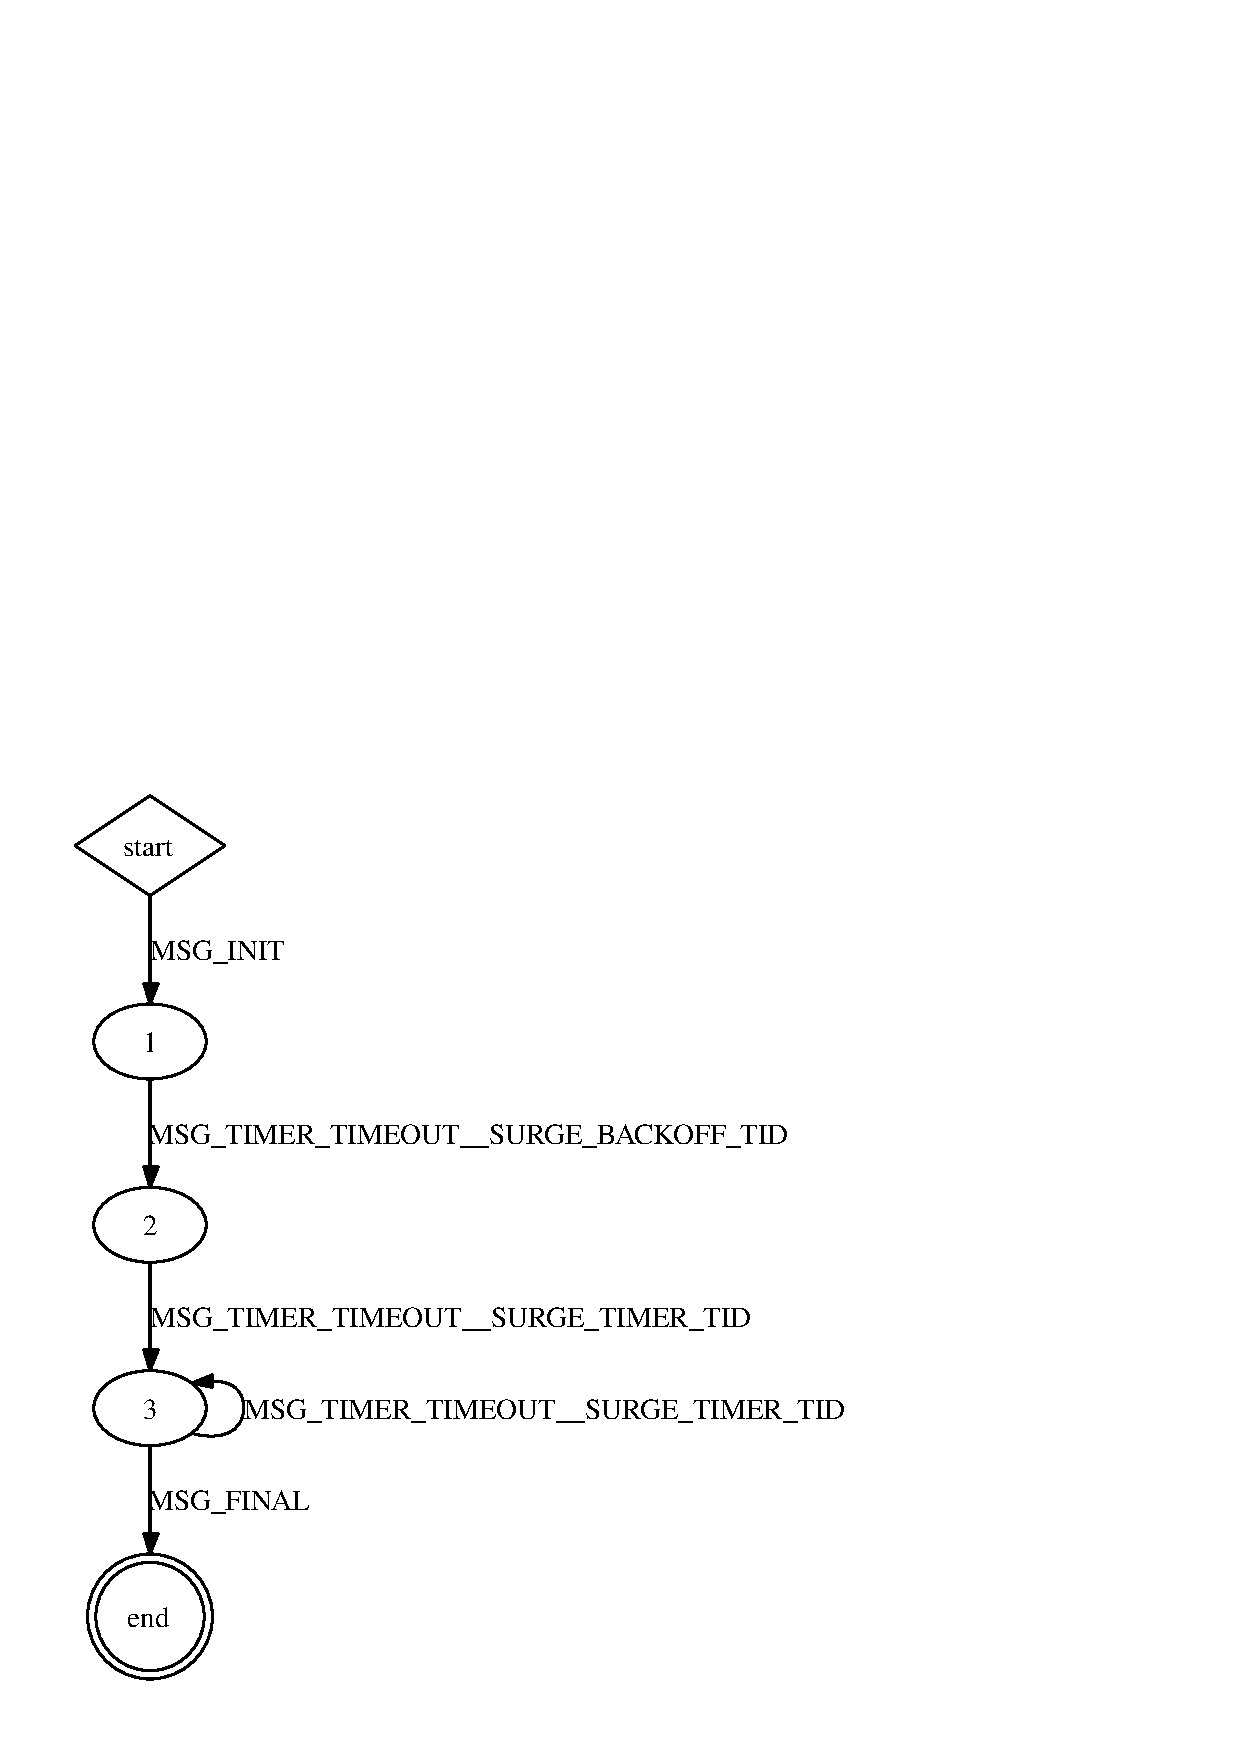
\includegraphics[angle=270,width=4.1in]{surge}
%\caption{{\tt surge} dataflow\label{fig:surge-dataflow}}
%\end{figure}


\subsection{Resource useage in {\tt surge}}

\begin{figure}[t]
\input{surge.c}
\caption{SOS implementation of {\tt surge}\label{fig:surge}}
\end{figure}

Figure~\ref{fig:surge} shows a portion of the SOS module that
implements {\tt surge}, a simple sensor network application that takes
sensor readings and sends the readings over a multihop network to a
base station~\cite{nesC}.  The function {\tt surge\_module} is the
entry point into {\tt surge} for messages from the kernel and from
other modules.  The function takes two arguments: a pointer to the
module's persistent state, which is saved in the kernel, and a pointer
to the current message.  A {\tt switch} statement is used to direct
each message type to an appropriate handler.  The handlers of interest
in this example are for the messages types {\tt MSG\_DATA\_READY} and
{\tt MSG\_TR\_DATA\_PKT}.

A sensor sends the message {\tt MSG\_DATA\_READY} to the surge module
when requested sensor data is ready to be read. The sensor data is
passed as the {\tt data} field of the message, which in general always
contains a message's payload.  Upon receiving this message, the {\tt
surge} message handler allocates a new packet ({\tt ker\_malloc}) to
be sent to the base station and posts a message ({\tt post\_long}) to
the tree-routing module in order to forward the sensor data.  The {\tt
post\_long} call is asynchronous, causing the kernel to package up all
the given arguments into a {\tt Message} structure and to schedule
this message for eventual delivery.

The message {\tt MSG\_TR\_DATA\_PKT} is sent by the tree-routing
module when data is received at the base station node.  Upon receiving
this message, the {\tt surge} message handler confirms that the
current node is the base station.  If so, the message handler forwards
the data to the UART driver via an asynchronous message send ({\tt
post\_net}).

The SOS kernel provides an API for programmers to manage dynamic
memory.  As shown in Figure~\ref{fig:surge}, the {\tt ker\_malloc}
function acts as expected, allocating a new block of memory.  The
kernel also provides a {\tt ker\_free} function for destroying
dynamically allocated memory.  Additionally, ownership of dynamic
memory can be transfered between modules through the messaging
interface provided in SOS.

%
% NOTE (ROY): This is not adding much to the discussion.  10-18-06
%
%In order to provide a simple form of automatic garbage collection for
%dynamically allocated memory, the SOS kernel imposes an {\em
%ownership} model on dynamic memory~\cite{sos}.  Each block of memory
%has a unique owner at any point in time, and the kernel maintains a
%mapping from each block of memory to its owner.  A block's initial
%owner is the module that allocates that block.  For example, the call
%to {\tt ker\_malloc} sets the {\tt surge} module as the initial owner
%of the newly allocated block.  When a module is removed from the
%system at run time, the kernel automatically frees all memory owned by
%that module.

Transfer of dynamic memory ownership occures at the end points of a
message.  First, the owner of a block of dynamically allocated memory
can explicitly {\em release} ownership of that block when it is passed
as the payload in a message.  This is accomplished by setting the
\texttt{SOS\_MSG\_RELEASE} flag in the corresponding {\tt post\_*}
call.  For example, the {\tt surge} module releases ownership of the
newly allocated {\tt pkt} upon sending it to the tree-routing module.
Second, a module can acquire ownership of a message's payload, which
is stored in the {\tt data} field, by calling
\texttt{ker\_msg\_take\_data} on an incoming message.  The function
returns a pointer to the message's payload.  For example, if the
current node is the base station, the {\tt surge} module explicitly
takes ownership of the given message's data under the name {\tt
payload}.

There are four release/take scenarios to consider.  If data is both
released by its sender and taken by its receiver, then ownership of
the data is transferred from the sender to the receiver.  If data is
released by its sender but not taken by its receiver, then the kernel
automatically frees the memory after the receiver's message handler
completes.  If data is not released by its sender but is taken by its
receiver, then the sender keeps ownership of the original message and
the receiver gains ownership of a new block of memory containing a
copy of that data.  Finally, if the data is not released by the sender
and not claimed by the receiver, then the sender keeps ownership of
the original message and the receiver has direct access to
``borrowed'' data for a limited period of time.  This last case is not
generally used in SOS due to the synchronization complications that
can result.


\subsection{Resource useage in {\tt GenericBaseM}}

\begin{figure}[t]
\input{surge.c}
\caption{TinyOS implementation of {\tt GenericBaseM recieve
interface}\label{fig:genericbase}}
\end{figure}


Figure~\ref{fig:genericbase} shows a portion of the TinyOS component
that implements the {\tt receive} event handler for {\tt GenericBaseM},
an application that uses a sensor node as a bridge between a base
station and the rest of a sensor network.  The {\tt receive} event
handler is passed in a {\tt TOS\_MsgPtr} pointing to the incoming
message and a flag describing where the message source.  If there are
no messages waiting to be sent, the handler forwards the message out
over the bridged interface and returns a pointer to a free message
buffer.  If a message is currently pending, the handler simply ignores
the message and returns the incoming message buffer to be reused.

A key property demonstrated by this TinyOS component is that of buffer
swapping.  Buffer swapping is throughout systems when dynamic buffer
creation is not desired or when dynamic buffer creation is simply not
allowed and is is a common technique used within TinyOS to allow data
to quickly pass through stacks of components.  Rather than
dynamicallyl allocating a new buffer, a call stack can simply return a
free buffer to the caller.  In the the TinyOS environment, handlers
that implement buffer swapping have implict memory ownership
responsibilities.  The handler can be though of needing to claim the
incoming {\tt TOS\_MsgPtr} and release a buffer to the caller.  Note
that this can be accomplished by returning the incoming buffer.


%%%%%%%%%%%%%%%%%%%%%%%%%%%%%%%%%%%%%%%%%%%%%%%%%%%%%%%%%%%%

\subsection{Static Ownership Checking}

SOS's original concept of ownership as described above provides
developers with a framework for designing modular programs. While this
can help reduce the complexity of managing dynamic memory, it is not
sufficient to prevent memory errors such as dangling pointers and
memory leaks.  For example, nothing prevents a module from freeing
some memory while another module (or even the same module) still has a
pointer to that memory.  If that pointer is ever accessed later, an
invalid dereference will result.  

A similar problem can occure with buffer swapping in TinyOS.  A TinyOS
component can improperly return a pointer to a buffer that is not yet
free during a buffer swap.  From that point on two components in the
system belive that they own the same buffer.  This leads to
unpredictable and unintional sharing of the buffer.

%
% NOTE: This depends on the garbage collection comment above
%
% Further, simple garbage collection introduces the potential for more
% dangling pointer errors, since the removal of a module implicitly
% frees the memory it owns, even if other modules have pointers to
% that memory.

In this work, we augment the often implicit ownership directives in
sensor network operating systems to provide a protocol governing
memory management that is sufficient to ensure the absence of memory
errors.  Our protocol makes explicit a common programming idiom in
sensor-network systems, whereby data is rarely shared but instead
follows a producer/consumer model.  We have built a tool that checks
for violations of this protocol on each SOS module at compile time.

Informally, the rules of the protocol can be stated as follows:
%
\begin{itemize}
%
\item A module may only manipulate the memory that it owns.
%
\item A module that takes ownership of a block of memory (either
through a function that allocates data or via a transfer of ownership)
must either free that memory, release it, or store it in the module's
persistent state.
%
\item A module may only free or release memory that it owns.  After a
module frees or releases memory, it may not access or update that
memory.
%
\end{itemize}
%
Because only the owner can manipulate or free its memory, dangling
pointers are avoided.  Because all memory must be either freed,
released or persistently stored by its owner, memory leaks are
avoided.


\subsubsection{Applying Ownership Protocol to {\tt surge}}

The {\tt surge} module described above can be showen to adhere to this
ownership protocol.  The {\tt MSG\_DATA\_RDY} message handler
allocates {\tt pkt} and takes ownership. This pointer is then
dereferenced in order to provide the sensor data to be sent up the
routing tree.  This pointer manipulation is safe since the module has
ownership.  The module then releases ownership by posting {\tt pkt} to
the tree routing module using the {\tt SOS\_MSG\_RELEASE} tag.  After
this release, the module does not access {\tt pkt} again and does not
store it, ensuring that access to the pointer is indeed released. 

The handler for {\tt MSG\_TR\_DATA\_PKT} also conforms to the
protocol.   When the current node is the base station, the handler
explicitly acquires ownership of the message's data using {\tt
ker\_msg\_take\_data}.  This allows the module to manipulate the data
and to pass it to the UART.  The {\tt post\_net} call explicitly
releases the data, fulfilling the module's obligation to that data.
After the release, the data is no longer accessed or stored.

While the {\tt surge} code is correct, small changes to the code can
easily cause problems to occur at run time, and our static checker
catches these potential errors.  For example, suppose the handler for
{\tt MSG\_DATA\_READY} did not release ownership of {\tt pkt} by
setting the {\tt SOS\_MSG\_RELEASE} flag in the call to {\tt
post\_long}.  In that case, the module would leak the memory allocated
for {\tt pkt}.  Indeed, our checker flags this modified version of the
code as erroneous, since {\tt surge} would not be freeing, releasing,
or storing the data for which it has taken ownership.


\subsubsection{Applying Ownership Protocol to {\tt GenericBaseM}}

It is also easy to show that the {\tt GenericBaseM} module follows the
ownership model described above.  Upon entry to the {\tt receive}
event handler the {\tt GenericBaseM} component owns the buffer
referenced by the global variable {\tt ourBuffer} and gains ownership
of the {\tt received} buffer passed into the function.  Within the
body of the function the handler, these are the only two buffers
accessed, although they are at times accessed via the alias {\tt
nextReceiveBuffer}.  At the end of the handler the buffer aliased by
{\tt nextReceiveBuffer} is returned to the calling function.  Note
that regardless of the path taken through the handler, at the call to
return the returned buffer is distinct from the buffer presistently
stored in {\tt ourBuffer}.  Thus the returned buffer is not accessed
by this component after the call to return.


\subsection{Function Attributes}

Our analysis is {\em modular}:  each function in a module or component
is analyzed in isolation.  To make checking of a function body precise
in the presence of calls to other functions, we employ {\em ownership
attributes} for function headers that capture the memory-related
behavior of a called function.  We add two attributes to the C code:
{\tt lh\_claim} and {\tt lh\_release}.  A formal parameter or return
value that has the {\tt lh\_claim} attribute indicates that the caller
must take ownership of the associated memory after a call.  This
annotation, for example, would be used to annotate a function that
wraps a call to {\tt ker\_malloc} within SOS, allowing that function's
callers to be properly checked without access to the function's
implementation.  Similarly, an {\tt lh\_release} attribute on a formal
parameter indicates that ownership of the parameter is transferred
from the caller of the function to the callee.  If a parameter does
not have an ownership attribute, memory ownership is unchanged.  Our
tool ensures that these attributes are employed wherever necessary,
when checking the implementation of each function.  In practice, we
have found that a small set of annotations is sufficient for precise
analysis.



\section{The Lighthouse Tool}
\label{sec:alg}



A discipline of {\em exclusive data ownership} underlies the examples
provided in section~\ref{sec:mot}.
%
References to resources are passed between multiple components to support
simple and efficient resource access.
%
However, only one component accesses a given resource at any point in time.
%
Each resource in this discipline has a unique owning component with the sole
capability to access the resource.
%
The owner also has the responsibility to eventually dispose of the resource or
explicitly transfer ownership to another component.



In this section we describe our approach to statically enforcing an exclusive
ownership discipline on sensor network applications.  
%
Informally, the following rules guarantee conformance to this discipline:
%
\begin{enumerate}
%
\item Each function may only refer to dynamic memory that it owns.  This
includes memory allocated in the function, memory accessible to the function
via global variables, and any formal parameters transferring dynamic data ownership to
the component.
%
\item Each function allocating or obtaining ownership of dynamic memory must
eventually free that memory, transfer its ownership to another component, or
store the memory in a persistent location.
%
\item A function may not access memory after freeing or releasing the memory.
%
\end{enumerate}



\subsection{TinyOS and SOS, Revisited}



The \code{SendMsg} interface described in section~\ref{ssec:tinyos} clearly
expects conformance to the above three rules.
%
Each component initially owns any \code{TOS\_Msg} that it declares.
%
Calls to the \code{send} command transfer ownership of the \code{TOS\_Msg}
from the component to the kernel, after which the component must not access
the message until ownership is regained via the \code{sendDone} event.
%
Interface contracts provide a means to verify these properties at {\em
run time}.
%
Our work describes a simple technique to {\em statically} examine these same
properties.
 


The SOS kernel already dynamically tracks memory ownership and has an
associated API for ownership transfer, which inspired our work.  
%
Tracked ownership enables the SOS kernel to perform basic garbage collection
when a module is removed from a node.
%
Calls to the messaging API can specify the \code{SOS\_MSG\_RELEASE} flag to
signal that ownership of the posted message is to be transferred to the callee
(or freed by the kernel if the callee does not explicitly take ownership).  
%
Calls to \code{ker\_malloc}, \code{ker\_free}, and \code{ker\_msg\_take\_data}
are known to allocate, free, and transfer ownership of memory respectively.
%
The SOS kernel only uses data ownership information when a module is removed
from a node at run time and assumes that the API manipulating memory ownership
is properly used.
%
Our work makes this protocol explicit and provides static checking for
conformance.



\subsection{Ownership Specification}


%  Use specification file
%  - documentation
%  - concise
%  - simlpe
%  - reusable
%  
%  Specification describes pre- and post- memory conditions for function
%  - full / empty
%  - formal / return / store
%  - Examples for malloc / free / post 
%  
%  Global store



Analyzing memory ownership requires understanding how functions manipulate
memory ownership properties.
%
Our analysis uses a simple specification file documenting functions that
transfer memory ownership between components.
%
Each function body is checked to ensure safety under the assumptions provided
by the specification.  



A function specification describes preconditions and postconditions to
denote expressions releasing memory buffers to or from the function.
%
Expressions in a specification may be one or more of: 
%
\begin{itemize}
%
\item Formal variable identified by its index in the function prototype
%
\item Function return value identified by the keyword \code{return} (only
valid in postconditions)
%
\item Global variable identified by variable name
%
\end{itemize}
%
An expression annotated with \code{release} in the precondition describes
dynamic memory that the caller is releasing to the callee, and therefore
that the function body must take ownership of.
%
An expression annotated with \code{release} in the postcondition describes
dynamic memory that the callee releases to the caller when the function
returns, and therefore that the function body must release.



\begin{figure}[tp]
\centering
\lstset{numbers=none, language=C}
\begin{lstlisting}
                ker_malloc.pre { $return.release; }
                ker_free.post { $1.release; }
\end{lstlisting}
\caption{\label{fig:spec}Specifications for \code{ker\_free} and
\code{ker\_malloc}.}
\end{figure}



Example specifications demonstrating these ideas are presented in
Figure~\ref{fig:spec}.
%
The postcondition qualifying the return statement with \code{release} notes
that the caller of \code{ker\_malloc} must take ownership of the returned
data.
%
The precondition qualifying the first formal parameter to \code{ker\_free}
with \code{release} specifies that it points to dynamic memory released from
the caller to the function body.



The specification resides in a single external configuration file.
%
Only functions requiring annotations need be included in the specifications.
%
In practice we have found that a small set of annotations, \numannote for
the complete evaluation of SOS, is sufficient for precise analysis. 



The specification allows modular checking by describing the side effects of
called functions.
%
The ability to perform modular checking allows application writers to obtain
early feedback about the correctness of their resource management, without
requiring access to the rest of the system.  
%
This is particularly important in a system like SOS, in which modules can be
linked and unlinked dynamically.  
%
In such a setting, the ``rest'' of the system is a moving target, so it is not
really possible to consider an approach based on whole-program analysis.



\subsection{Implementation Overview}



Lighthouse is implemented in the CIL front end for C~\cite{CIL}, which
parses C code into a simple intermediate format and provides a framework for
performing analysis on the intermediate code. 
%
Lighthouse takes as input a preprocessed C file and prints out warning
messages similar to those produced by a C compiler when suspect code is
identified.
%
The analysis does not modify the preprocessed code, so it can be trivially
called from a makefile between the preprocessing and code generation stages
of compilation.



Lighthouse uses a dataflow analysis to track the state of all expressions that
may alias dynamic memory within a function.
%
The dataflow ensures that:
%
\begin{itemize}
%
\item Whenever a node in the control flow graph is encountered that allocates
or takes ownership of a block of memory, every path from this node to the
function exit frees, stores, or releases ownership of the memory exactly once.  
%
If this property is not satisfied, Lighthouse reports a possible memory leak.
%
\item Whenever a node in the graph is encountered that frees or releases
ownership of a block of memory, that no path from this node to the function
exit accesses the memory.  
%
If this property is not satisfied, Lighthouse reports a possible dangling
pointer error.
%
\end{itemize}
%
For the purpose of the Lighthouse traversal over a function's CFG, the
function's entry node is considered an allocation point for all
parameters qualified as with \code{release} in the precondition, and the function's exit
nodes are considered release points for expressions qualified with
\code{release} in the postcondition.



The analysis described above requires knowledge of the memory pointed to by
a function's pointers.  
%
This is statically approximated by an alias analysis, which determines
whether two different pointers store the same memory location at a given
program point.  
%  %
%  Two standard approximations to the true dynamic alias information are {\em
%  must-alias} analysis and {\em may-alias} analysis.
%  %
%  We have built a simple flow-sensitive must-alias analysis for use by
%  Lighthouse.  
%  %
%  For the may-alias analysis, we use a fast flow-insensitive analysis provided
%  by the CIL framework.  
%  %
%  Obtaining precise alias information at compile time is notoriously
%  difficult, and this limitation is the principal cause of false positives for
%  our analysis.
%  %
%  For example, CIL's may-alias analysis does not distinguish among the fields
%  of a structure, instead considering them to always potentially alias one
%  another.  
%  %
%  Both alias analyses can be imprecise in the presence of linked data
%  structures.



\subsection{Limitations}



As we demonstrate in the next section, our checker is useful for detecting
violations of the ownership protocol on real sensor network code.  
%
However, the checker is not guaranteed to find all such violations.  
%
By favoring simplicity, scalability, and practicality, the checker allows some
false negatives.




First, we favored using a simple memory model at the cost of not precisely
handling all of the unsafe features of the C programming language.  
%
For example, pointer arithmetic is not statically analyzed.  
%
Instead, an expression of the form $p+i$, where $p$ is a pointer and $i$ is an
integer, is simply treated as if it refers to the same block of memory as $p$.  
%
If $p+i$ in fact overflows to another block of memory at run time, the
checker's assumption can cause it to miss errors.  
%
These kinds of memory safety assumptions are standard for C-based program
analysis.



Second, there is a design choice about how to treat dynamic memory referenced
by formal parameters without the \code{release} denotation.
%
Technically the ownership protocol disallows this memory from being accessed
at all, since the receiving component is not the owner.  
%
Lighthouse assumes a more practical stance by not enforcing the requirement
that a component only access a resource that it owns.
% 
This decision provides a mechanism for allowing patterns of resource sharing
that are in fact safe but not supported by the ownership discipline, for
example when a component temporarily ``borrows'' data from another component
within a bounded scope.
%
The cost of this flexibility is the potential to miss real resource management
errors.
%
However, the checker still ensures that a function does not access a resource
that has earlier been released by the function, thereby detecting memory
leaks.



Third, sensor network systems are often event driven by unpredictable event
orderings.
%
Our modular checker makes optimistic assumptions about the order of events
received by a component.  
%
However, event ordering affects the correctness of ownership tracking when a
memory accessed through a global variable.
%
For example, consider a component that responds to three events: $\create$
causes the component to allocate a block $b$ and store it into a global
store, $\access$ causes the component to access block $b$ via the store, and
$\delete$ causes the component to deallocate block $b$ from the global.  
%
The component avoids dangling accesses to $b$ and leaks of $b$ as long as
the temporal sequence of events follows the regular expression $($ $\alloc$
$\access^*$ $\delete$ $)^*$.  



Preferring a modular analysis that only requires examining a single function
at a time, Lighthouse only tracks data locally within each event handler.  
%
When performing this tracking, the tool assumes on entry that all data in
global stores is owned by the component.
%
The tool similarly considers a resource to be properly released when it is
placed in a global store.  
%
These assumptions allow each of the three event handlers in our example to
pass all checks.  
%
Nonetheless, dynamic memory errors can still happen, for example if an
$\access$ event ever occurs before the $\alloc$ event.  
%
Our assumptions provide a practical point in the design space that allows each
event handler to be usefully checked for local violations of the ownership
protocol.  



We have explored and implemented a prototype system combining Lighthouse with
a finite state machine (FSM) representation of the expected event orderings.
%
This allows tracking of global store state across event handlers, solving
the problem described above.
%
However, this requires pushing basic monitoring into the system run time to
watch for invalid event firing orders.
%
In practice, we found very few instances where the additional tracking of event
orderings helped refine our analysis of memory management in SOS.
%
More complete handling of inter-component relationships and application-level
protocols is something we plan to pursue in the future, leveraging recent work
on {\em interface synthesis} for software components~\cite{AlurPOPL05,HJM05}.


\section{Evaluation}
\label{sec:eval}

We evaluated our tool using the public CVS archives of the SOS
operating system.  SOS applications are made up of user modules that
run on a core kernel supplied by the operating system.  In this
analysis we ran the checker on individual modules and parts of the SOS
kernel to examine its utility in locating bugs.  

\subsection{Quantifying Dynamic Memory Usage in SOS}

Of interest is the prevalence of dynamic memory operations in the SOS
applications.  The SOS API includes a number of functions that
manipulate memory.  These functions are used to allocate, free, and
transfer ownership of blocks of memory.  To quantify the use of these
functions within SOS, we examine the frequency of memory
manipulation functions by user modules. 

The CVS head from October 2006 reveals 36 modules totaling 5824 lines
of source code.  Within this sample there are 178 lines of code
calling a function that manipulates memory.  This is about one such
function call for every 32 lines of code.  Similarly, looking at all
historic version of all SOS modules reveals a similar density of
function calls.  These findings indicate that memory management has
been and continues to be an important part of resource management in
SOS.


\subsection{Validating SOS End-User Modules}

Next we ran our tool on all SOS end-user modules from the October 2006
head of the SOS CVS repository.  The goal of this experiment was to
demonstrate that the tool is practical for use as part of the standard
development cycle and to demonstrate its ability to locate errors in
real sensor-network software.  For this analysis, we only consider the
first occurrence of a particular bug withing a program, even if the bug
lasts through multiple consecutive versions of a particular module.


The checker can be easily added to the normal build process of a C
application.  It takes as input a preprocessed C file and generates
warnings similar to those generated at other stages of compilation.
The analysis generates two types of warnings:
%
\begin{description}
%
\item[Memory leak:] Source code neither stores, releases, nor frees
data that was taken or allocated.
%
\item[Dangling pointer:] Source code is accessing data that was
released or freed at an earlier point.
%
\end{description}


\begin{table}
\caption{Warnings in SOS user modules}
%
\label{tab:module}
\centering 
\begin{tabular}{| l | r |}
    \hline 
    Verified memory leaks identified by analysis & 8 \\
    \hline
    False memory leaks identified by analysis & 8 \\
    \hline 
    Verified dangling pointers identified by analysis & 0 \\
    \hline 
    False dangling pointers identified by analysis & 9 \\
    \hline 
\end{tabular} 
%
\end{table}

We applied the checker to every historic version of each user module
included in the SOS CVS repository that would compile for the
\code{mica2} target.  
%
Of the 213 historic versions of the 48 modules available, new warnings
appeared in 13 versions.  For this analysis we only counted the first
occurrence of a bug, even if it persisted through multiple versions of
a module.
%
An external configuration of 24 function annotations was used for this
analysis.  Additionally, local store annotations were added to 9
module versions and a change to the core SOS API from the summer of
2006 required changing the value of a constant in 6 module versions.


A total of 25 warnings were generated by the checker during this
experiment.  Each warning was examined by hand and classified as an
actual error or a false positive; the results are presented in
Table~\ref{tab:module}.  Eight of the warnings turned out to be real
memory leaks in the code.  An example memory leak from the code is
described at the end of this section.
%
The 17 remaining warnings were further classified to better
understand the sources of imprecision in the current implementation of
the checker.  


\smallskip\noindent{\bf Memory leak false positives.}

False positive memory leaks came from two different sources. Five of
the false positives resulted from a conservative assumption made by
the must alias analysis used within the checker.  The analysis assumes
that functions can change what data is referenced by a formal
parameter.  This results in the must alias information being lost in
these cases.  The analysis can easily rank these as probable false
positives if the end user wishes to see more likely errors first.

The other three memory leaks are the result of linked list data
structures that the must alias analysis is unable to properly reason
about.  

\smallskip\noindent{\bf Dangling pointer false positives.}

The nine dangling pointer false positives result from limitations of
the flow-insensitive and field-insensitive analysis.  A benefit of the
sensor network domain is the limited scope of program components.
This opens the door to using context sensitive analysis that suffer
from scaling limitations in more general domains.



\subsection{Validating the SOS Kernel}

\begin{table}
\caption{Warnings in the SOS kernel}
%
\label{tab:kernel}
\centering 
\begin{tabular}{| l | r |}
    \hline 
    Verified memory leaks identified by analysis & 2 \\
    \hline
    False memory leaks identified by analysis & 22 \\
    \hline 
    Verified dangling pointers identified by analysis & 0 \\
    \hline 
    False dangling pointers identified by analysis & 11 \\
    \hline 
    \hline 
\end{tabular} 
%
\end{table}


We ran a similar experiment on the SOS kernel.  We ran the checker on
the current version of all code required to build the core SOS kernel
with a simple ``blank'' application for the Mica2 hardware.  This
configuration consists of approximately 9000 lines of source code and required
analyzing 40 source files, of which 35 generated warnings.  A detailed
listing of these warnings is provided in table~\ref{tab:kernel}.

The two actual memory leaks represent an interesting type of error.
These leaks resulted from functions that would released a formal
parameter, except in exceptional cases where an error code is returned
to the user.  One could argue that these functions do not leak memory,
but rather conditionally release memory.  We opted for classifying
them as errors, since user code did not bother to check return values
for the conditional release of data.  We could have changed the
analysis to treat these functions as conditional releases.  In this
case the two functions would not have been found to be in error, but a
number of additional bugs would have been located in the user code.

A second point of interest are the different rates of false positives
reported for user modules and for the kernel.  User modules resulted
in approximately one false positive for every 1650 lines of source
code.  The kernel saw a much higher frequency at approximately one 
false positive for every 270 lines of source code.  

A large contributor to this increased rate of false positives within
the kernel are the ``bottom layer'' functions implementing management
of memory in SOS.  These functions manipulate memory in a manner that
does not conform to the model assumed for the analysis.  For example,
the function \code{ker\_msg\_take\_data} is annotated to denote that
it returns dynamically allocated memory.  When the analysis examines
the function to confirm that this is the case, it generates an error
declaring that the function does not return dynamically allocated
memory.  This is because the function directly accesses the internal
data structures of the SOS memory manager to return a pointer to
dynamically allocated data, rather than using an annotated interface
such as \code{ker\_malloc}.


% ROY (11/04/06):
% This does not seem to stand on its own.  For now I will simply leave
% the allision to this challenge as a point for the conclusion.
%
% \subsection{Comments}
% 
% A third source of false positives arises from application-level
% protocols that ensure memory is used correctly across multiple
% invocations of the module's message handler, but which cannot be
% validated modularly.

\subsection{A Memory Leak in SOS}
\label{ss:tale}

\begin{figure}[tp]
\begin{footnotesize}
\begin{verbatim}
mod_op = (sos_module_op_t*) ker_msg_take_data(msg);
if(mod_op == NULL) return -ENOMEM;
if(mod_op->op == MODULE_OP_INSMOD) {
    existing_module = ker_get_module(mod_op->mod_id);
    if(existing_module != NULL) {
        uint8_t ver = sos_read_header_byte(
                existing_module->header,
                offsetof(mod_header_t, version));
            if (ver < mod_op->version) {
                ker_unload_module(existing_module->pid, 
                        sos_read_header_byte(
                        existing_module->header,
                        offsetof(mod_header_t, version)));
            } else {
                return SOS_OK;
            }
        }
    ret = fetcher_request(KER_DFT_LOADER_PID,
            mod_op->mod_id,
            mod_op->version,
            entohs(mod_op->size),
            msg->saddr);
    s->pend = mod_op;
    ker_led(LED_RED_TOGGLE);
    return SOS_OK;
}
return SOS_OK;
\end{verbatim}
\end{footnotesize}
\label{fig:leak}
\caption{A memory leak in an SOS module.}
\end{figure}

This section examines the SOS loader, a core part of SOS that allows
users to dynamically add modules to a running system and that is
known to have caused stability problems for developers in the past.
We used the checker to see if such a tool could have eased development
pains.

In mid-October 2005 the block of code shown in Figure~\ref{fig:leak}
was checked into CVS as part of {\tt loader.c} and introduced a memory
leak into the loader.  All paths through this block of code leak the
{\tt mod\_op} pointer, which the module acquires ownership of through
{\tt ker\_msg\_take\_data}.  This code results in the following
warning from the checker:

\begin{footnotesize}
\begin{verbatim}
Error: Expression mod_op is not stored after instruction #line 125
mod_op = (sos_module_op_t *)ker_msg_take_data((unsigned char)18, msg);
\end{verbatim}
\end{footnotesize}

After three additional revisions that do not significantly modify or
fix the memory leak, a fourth revision was made in mid-December 2005.
This revision expands the functionality of {\tt loader.c} and breaks
the code up into smaller functions:

\begin{footnotesize}
\begin{verbatim}
sos_module_op_t *mod_op;
if (msg->saddr == ker_id() || s->pend) {
    return SOS_OK;
}
mod_op = (sos_module_op_t*) ker_msg_take_data(msg);
if(mod_op == NULL) return -ENOMEM;
switch(mod_op->op){
case MODULE_OP_INSMOD:
    return module_op_insmod(s,msg,mod_op);
case MODULE_OP_RMMOD:
    return module_op_rmmod(s,msg,mod_op);
}
return SOS_OK;
\end{verbatim}
\end{footnotesize}

This code again causes our checker to warn about the memory leak:

\begin{footnotesize}
\begin{verbatim}
Error: Expression mod_op is not stored after instruction #line 186
mod_op = (sos_module_op_t *)ker_msg_take_data((unsigned char)18, msg);
\end{verbatim}
\end{footnotesize}

Clearly {\tt mod\_op} is still being leaked if {\tt mod\_op->op} does
not find a matching case in the {\tt switch} statement.  Further,
adding the {\tt sos\_release} attribute to the third formal parameter
of the functions {\tt module\_op\_insmod} and {\tt module\_op\_rmmod}
and rerunning the checker reveals that both of these functions also
leak {\tt mod\_op}!

A day later, eight weeks after the memory leaks were first introduced,
these memory leaks were found and fixed:

\begin{footnotesize}
\begin{verbatim}
sos_module_op_t *mod_op;
if (msg->saddr == ker_id() || s->pend) {
    return SOS_OK;
}
mod_op = (sos_module_op_t*) ker_msg_take_data(msg);
if(mod_op == NULL) return -ENOMEM;
switch(mod_op->op){
case MODULE_OP_INSMOD:
    return module_op_insmod(s,msg,mod_op);
case MODULE_OP_RMMOD:
    return module_op_rmmod(s,msg,mod_op);
}
ker_free(mod_op);
return SOS_OK;
\end{verbatim}
\end{footnotesize}

As shown above, a call to {\tt ker\_free} has been added before the
final {\tt return}, in order to properly dispose of {\tt mod\_op}.
The functions {\tt module\_op\_insmod} and {\tt module\_op\_rmmod}
similarly free their third argument.  The CVS log message simply reads
``fixed another memory leak.''






\section{Related Work}
\label{sec:related}

\subsection{Sensor Network Analysis Research}

The memory manager in the SOS operating
system~\cite{sos} performs basic memory ownership tracking to clean
the system after module removal.
%
However, the burden remains on the end user to prevent memory leaks in
active modules and to not dereference invalid pointers.
%
Our work grew out of a desire to prevent these kinds of errors from
occurring in SOS applications.



Dynamic checking of sensor network systems has become a popular technique to
improve system reliability and find system errors.
%
Recent work on Safe TinyOS, UTOS~\cite{regehr06memory} and software fault
isolation for embedded processors~\cite{kumar07system} uses static analysis
to insert run-time checks ensuring memory protection for sensor-network
systems.
%
Interface contract monitoring~\cite{archer07interface} interposes a thin
layer between interface clients and implementers, and has proved effective
in finding bugs in TinyOS programs.
%
These approaches provide valuable feedback to developers when an executing
system misbehaves.
%
In contrast to these works, the static analysis in Lighthouse focuses on
alerting developers to problems at compile time.



Sensor network platforms include support for static checking targeting
other classes of errors.  
%
The nesC~\cite{nesC} language used in TinyOS employs a whole-program
analysis to statically detect race conditions and
galsC~\cite{TinyGALS,galsC} employs an analysis to ensure the type safety of
connections between components.  



A complementary approach to improving the reliability of sensor network
software is through new language abstractions.  
%
Researchers have explored language support for component-based
programming~\cite{TinyOS,nesC,galsC}, region
abstractions~\cite{conf/mobisys/WhitehouseSCB04,conf/nsdi/WelshM04},
component composition~\cite{conf/sensys/GreensteinKE04}, and programming in
the aggregate~\cite{1052213,conf/dcoss/GummadiGG05}.
%
New language constructs enable easier expression of certain programming
idioms, often making programs more amenable to static checking.  
%
Our tool currently analyzes ordinary C programs, since that is the language
that SOS employs, but it would be interesting to explore ways to leverage
specialized language constructs to improve the tool's effectiveness.



\subsection{Traditional Systems Analysis Research}



Static analysis has long been used to find bugs in traditional systems.
%
Dedicated languges, such as Metal~\cite{engler00checking}, are used to
compose custom compiler extensions to verify properties at compile time.
%
Such properties can even be infered from the code
itself~\cite{kremenek06from}.
%
Clouseau~\cite{heine03practical} ensures that dynamically allocated memory
is freed exactly once in C and C++ programs.
%
The whole program analysis provided by Clouseau uses a constraint system to
track owning pointers both intra- and inter-procedurally.
%
A key diffrence in our work is our focuses to create an understandable
programing discipline, accomplished using explicit lightweight
specifications that increase developer vilibility into the analysis and
obviate the need for interprocedural analysis.
%
Other technical differences also exist.
%
Where Metal ignores aliasing, Lighthouse provides a stronger analysis
explicitly consedering aliases.
%
Unlike Clouseau, our work detects dangling pointers.




Recent work in the programming languages community explores the concept of
ownership types~\cite{ownership,ownership2,BoyapatiEtAl02,aliasjava} for
object-oriented languages. 
%
Ownership types designate an owner object for each object, and the static
type system ensures access to an object goes through its owner.
%
Related work on confined types~\cite{confined1,confined2} provides a more
static form of confinement, in which an object is guaranteed not to escape a
particular static scope.



Our work provides a static notion of ownership analogous to that of confined
types:  all accesses to a given resource may only occur within the static
scope of its owning module.  
%
On a technical level, however, the foundation of our work is quite distinct
from that of both ownership types and confined types, as we rely on dataflow
analysis rather than on type systems.  
%
Our use of dataflow analysis is necessary in order to safely accommodate
dynamic transfer of ownership, which the systems described above lack.  
%
Ownership transfer is critical in practice for sensor network applications,
for example it is needed to properly account for split-phase operations.  
%
Although recent work has explored a form of transfer in the context of
ownership type systems~\cite{DBLP:conf/ecoop/BanerjeeN05}, that work
requires programmers to provide detailed assertions about ownership, and
these assertions are proved as part of a more general program specification
and verification framework.



There have been several proposals for a form of {\em unique} or {\em linear}
pointer~\cite{Boyland:2001:ABU,aliasjava,Wad90:linear}, which is guaranteed
to be the only reference to its referent.  
%
These systems sometimes include a form of transfer of uniqueness from one
pointer to another.
%
For example, a {\tt unique} pointer in AliasJava~\cite{aliasjava} can be
transferred as long as a dataflow analysis shows that the original pointer
is no longer accessed after the transfer.  
%
Our tool does not enforce a uniqueness requirement.
%
Instead, a resource may have any number of aliases from within its owning
component, which is less restrictive and sometimes necessary in practice.
%
At the same time, transfer is still safely allowed, as long as none of these
aliases are accessed after the transfer.



A language extension to C\# called Sing\# provides a {\em channel} construct
for message-based communication, and the Singularity operating system uses
Sing\# channels for communication among
processes~\cite{fahndrich06language}.  
%
Sing\# employs a type system for channels based on the Vault
language~\cite{Vault,adoption-focus}, which provides a sophisticated form of
linear types, to enforce ownership invariants on data buffers passed among
processes.  
%
This includes the use of programmer-defined channel {\em contracts} to
specify and check ownership transfer.
%
Lighthouse enforces a similar ownership discipline on dynamic memory in SOS,
but at a very different point in the design space.  
%
Rather than devising a new language and type system, our approach works
seamlessly with standard languages and tool chains for sensor-network
programming in a lightweight manner.  
%
Of course, a language solution like Sing\# has the potential to be more
expressive and to provide stronger guarantees, by enforcing a stylized
programming model.



\section{Conclusion}
\label{sec:conc}

Systems programming APIs for networked embedded systems applications
are getting more expressive as the applications become more
sophisticated.  This necessitates a programming environment that
supports program development by providing automated compile-time
checkers for proper API usage.  Such verification support is
particularly important in the sensor network domain.  First,
programmers are often domain experts who may not be systems
programming experts. Second, the cost of fixing a bug in the field is
high.  Third, networked embedded systems come with somewhat limited
debugging support, making it extremely difficult to reason about the
cause for a failure in the field.

This paper is our first step toward providing static analysis tools
that capture common programming idioms in networked embedded systems.
We have focused on dynamic resource management initially, since our
experience with SOS suggests that improper memory management is a
common source of hard-to-debug problems.  We have demonstrated how our
checker can effectively find memory errors even in code written by
systems experts.  Our memory checker is now provided as part of the
SOS development environment; it is invoked automatically in the build
process.

In the future, we would like to augment the techniques in this paper
with support for reasoning about application-level protocols
\cite{AlurPOPL05,HJM05} as well as concurrency issues.  Ultimately,
our goal is to provide a systems programming environment where many
common classes of bugs are automatically detected at compile time.  We
believe such early feedback will help increase the productivity of
sensor network programmers and the reliability of their software.




{\small 
\bibliographystyle{abbrv}
\bibliography{sw,sos,references}

}

\end{document}


